\documentclass{beamer}
\usepackage{tikz}
\usepackage{lmodern}% http://ctan.org/pkg/lm
\usepackage[utf8]{inputenc}
\usetheme{Warsaw}

\title{Missing Values}
\subtitle{A thorn in the side}
\author{Thomas LOUIS}\institute{Data scientist}

\begin{document}

\begin{frame}
\titlepage
\end{frame}

\begin{frame}
	\begin{center}
	\Huge Why this presentation ?
	\end{center}
\end{frame}

\begin{frame}
  \begin{tikzpicture}[remember picture,overlay]
   \node[at=(current page.center)] {
     
\includegraphics[width=\paperwidth]{22ftbs.jpg}
     };
  \end{tikzpicture}
\end{frame}

% Give examples :
%
% - Poll, people don't answer to every questions => Studies / Research
% - Customer information are rarely complete => recommandation system
% - Technical issues can occur without warnings and you can't recover past data.
% ONE INDUSTRY EXAMPLE
%

\begin{frame}
\frametitle{Introduction}
	\framesubtitle{Missing values in Data Driven Business}
	Why am I talking about missing values ?
        \begin{enumerate}
		\item<1- | alert@1> Because it's everywhere.
		\item<2- | alert@2> Dealing with missing values is tricky and could lead to disasters  
		\item<3- | alert@3> It's interesting
	\end{enumerate}
\end{frame}

\begin{frame}
  \frametitle{Introduction}
  \framesubtitle{A definition of missing values/data}
  \textsc{Missing values}, what is it ?
  \begin{quote}
  Wikipedia : In statistics, missing data, or missing values, occur when no data value is stored for the variable in an observation. Missing data are a common occurrence and can have a significant effect on the conclusions that can be drawn from the data
  \end{quote}
  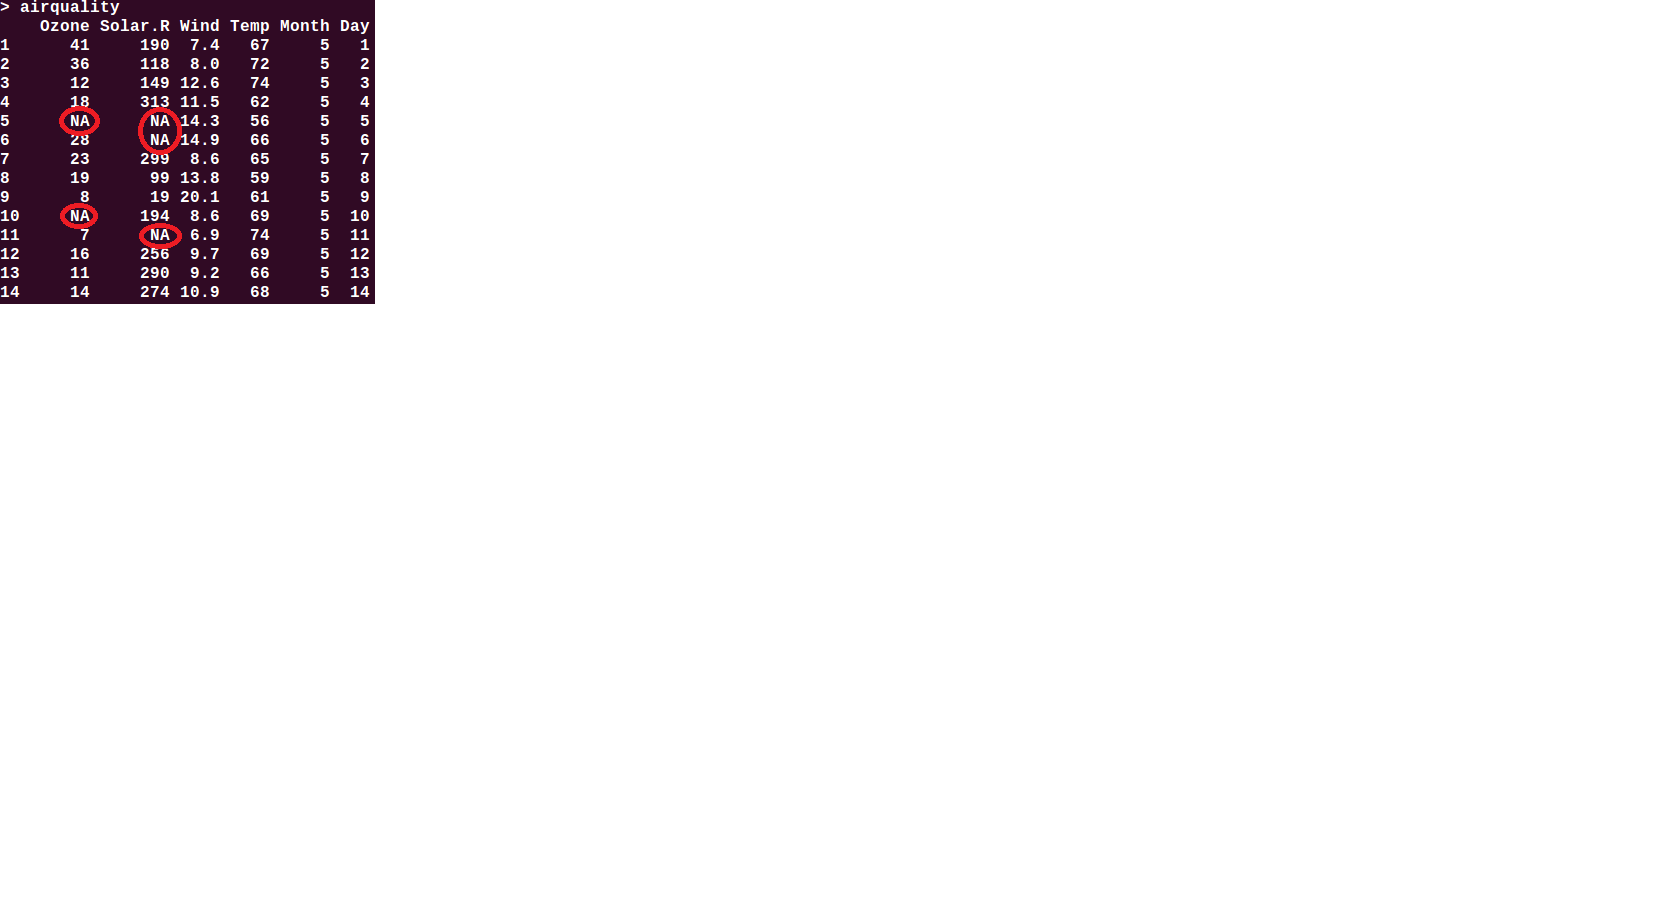
\includegraphics[width=25cm]{missingvalues.png}
\end{frame}

\begin{frame}
  \frametitle{Introduction}
  \framesubtitle{Dealing with missingness is a science}

  \begin{enumerate}
      \item<1- | alert@1> 
  \end{enumerate}

  
\end{frame}

\begin{frame}
  \frametitle{References}
	\begin{itemize}
		\item<1->Constructing Models to Deal With Missing Data | SciPy 2016 | Deborah Hanus, https://www.youtube.com/watch?v=cHzahWjaA7o
	\end{itemize}
\end{frame}


\end{document}

% some references :
% - Constructing Models to Deal With Missing Data | SciPy 2016 | Deborah Hanus, https://www.youtube.com/watch?v=cHzahWjaA7o
% - http://www.bias-project.org.uk/papers/NonTechnicalMissingTalkSlides.pdf
